% =====================================================================
\section{Practice: Graph-Identification Items}\label{ch:drills}
% =====================================================================

Try each item using the checklists from Chapters~\ref{ch:curves}--\ref{ch:idfields} before
looking at the answers at the end of the chapter.

\subsection*{Picture items}

\textbf{1.} Which curve is $\vr(t)=\ip{t\cos t,\ t\sin t,\ t}$, $t\ge0$?
\begin{center}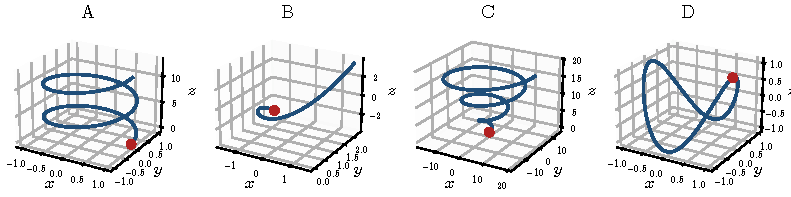
\includegraphics[width=0.95\linewidth]{drill_curves}\end{center}

\textbf{2.} Which curve is $\vr(t)=\ip{\cos t,\ \sin t,\ 2-\sin t}$, $0\le t\le2\pi$?
(The red dot is the point at $t=0$.)
\begin{center}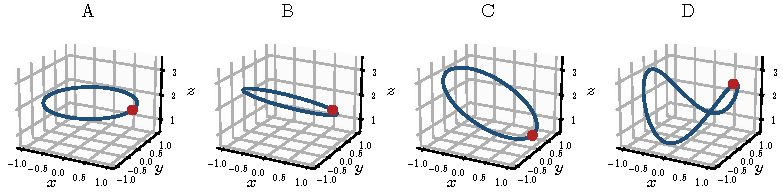
\includegraphics[width=0.95\linewidth]{drill_curves2}\end{center}

\textbf{3.} Match each field with its plot I--IV:\quad
(a) $\ip{x,-y}$\quad (b) $\ip{1,x}$\quad (c) $\ip{y,-x}$\quad (d) $\ip{-x,-y}$.
\begin{center}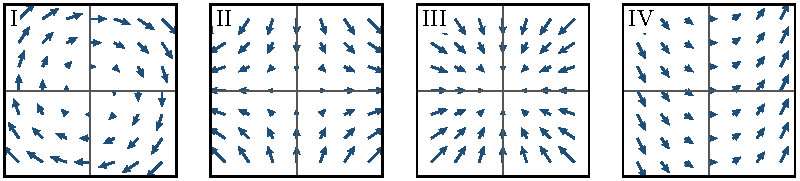
\includegraphics[width=0.95\linewidth]{drill_fields}\end{center}

\textbf{4.} Which plot is the gradient field of $f(x,y)=x^2y$? (All arrows are drawn with the
same length; only the directions matter.)
\begin{center}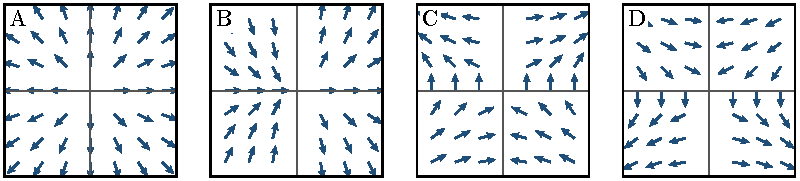
\includegraphics[width=0.95\linewidth]{drill_gradient}\end{center}

\textbf{5.} The contour map of $f$ is shown below (levels labelled).
\begin{center}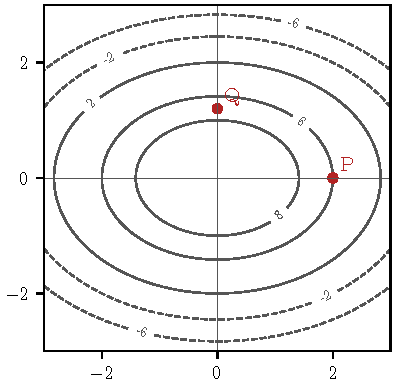
\includegraphics[width=0.36\linewidth]{drill_contour}\end{center}
(a) Is $D_{\vi}f(P)$ positive, negative or zero?\quad
(b) In which direction does $\grad f(Q)$ point?\quad
(c) Give a unit vector $\vu$ with $\Du f(P)=0$.\quad
(d) Does $f$ have a maximum or a minimum at the origin?

\subsection*{Formula-only items}

\begin{enumerate}[label=\textbf{\arabic*.},start=6]
\item Which curve lies on the cone $z^2=x^2+y^2$?\\
  A.\ $\ip{\cos t,\sin t,t}$\quad B.\ $\ip{t\cos t,t\sin t,t}$\quad C.\ $\ip{t,t^2,t^3}$\quad D.\ $\ip{\cos t,t,\sin t}$
\item Viewed from above, $\vr(t)=\ip{\sin t,\cos t,t}$ starts at \underline{\hspace{2cm}} and turns
  \underline{\hspace{2.5cm}}.
\item The helix $\ip{t,\ 3\cos t,\ 3\sin t}$ winds around which axis?
\item The curve $\ip{\cos^2t,\ \sin^2t,\ t}$ lies in which plane?
\item Which curve has curvature $0$ everywhere?\\
  A.\ $\ip{2t,1-t,3+4t}$\quad B.\ $\ip{t,t^2,0}$\quad C.\ $\ip{\cos t,\sin t,0}$\quad D.\ $\ip{t,t^3,t}$
\item Which field is conservative?\\
  A.\ $\ip{-y,x}$\quad B.\ $\ip{y,x}$\quad C.\ $\ip{y,-x}$\quad D.\ $\ip{x^2,xy}$
\item A plot shows arrows tangent to circles about the origin, turning counterclockwise and
  getting \emph{shorter} away from the origin. Which field?\\
  A.\ $\ip{-y,x}$\quad B.\ $\ip{y,-x}$\quad C.\ $\dfrac{\ip{-y,x}}{x^2+y^2}$\quad D.\ $\dfrac{\ip{x,y}}{x^2+y^2}$
\item Domain of $\vr(t)=\ip{\sqrt{4-t^2},\ \ln t,\ \dfrac1{t-1}}$?
\item A plot shows every arrow pointing straight up or straight down, up for $x>0$ and down for
  $x<0$. Which field?\quad A.\ $\ip{x,0}$\quad B.\ $\ip{0,x}$\quad C.\ $\ip{0,y}$\quad D.\ $\ip{y,0}$
\end{enumerate}

\subsection*{Answers}

\begin{enumerate}[label=\textbf{\arabic*.}]
\item \textbf{C.} $x^2+y^2=t^2=z^2$: a cone, so the spiral widens as it climbs. A has constant
  radius (ordinary helix), B is the twisted cubic, D is a closed loop.
\item \textbf{B.} At $t=0$ the point is $(1,0,2)$, which rules out C (starts at $z=1$) and D
  (starts at $z=3$). $z$ is not constant, which rules out A. Also $z=2-y$: highest at $y=-1$, so the
  loop is tilted along the $y$-direction, as in B.
\item (a) \textbf{II}, (b) \textbf{IV}, (c) \textbf{I}, (d) \textbf{III}.
  Test points: $\ip{y,-x}$ at $(0,1)$ is $\ip{1,0}$ (right, on top), so clockwise: I.
  $\ip{-x,-y}$ points inward: III. $\ip{x,-y}$ at $(1,0)$ points right but at $(0,1)$ points
  down: saddle, II. $\ip{1,x}$ always has $M=1$ (rightward) and tilts up for $x>0$: IV.
\item \textbf{C.} $\grad f=\ip{2xy,\ x^2}$. Its $y$-component $x^2\ge0$, so no arrow points
  down (rules out D), and on the $x$-axis ($y=0$) the arrows point straight up. A is
  $\grad(x^2+y^2)$ (radial); B has the components swapped ($\ip{x^2,2xy}$ always points right).
\item (a) \textbf{Negative}: moving right from $P$ goes to lower contours (6, then 2).
  (b) Straight \textbf{down}, toward the origin: perpendicular to the level curve and toward
  larger values (here $f=10-x^2-2y^2$, so $\grad f(Q)=\ip{0,-4.8}$). (c) $\vu=\pm\vj$ (tangent
  to the level curve at $P$). (d) A \textbf{maximum}: the levels increase toward the centre.
\item \textbf{B.}
\item $(0,1,0)$; \textbf{clockwise}.
\item The \textbf{$x$-axis} ($x=t$ is the variable that appears alone).
\item $x+y=\cos^2t+\sin^2t=1$: the plane \boldmath$x+y=1$\unboldmath.
\item \textbf{A} (all components linear, so it is a line).
\item \textbf{B.} $M_y=1=N_x$; potential $f=xy$. (A and C rotate; D: $M_y=0\ne y=N_x$.)
\item \textbf{C.} The length is $r/r^2=1/r$, so it shrinks; A grows, B is clockwise, D is radial.
\item Need $4-t^2\ge0$, $t>0$, $t\ne1$: \ \boldmath$(0,1)\cup(1,2]$\unboldmath.
\item \textbf{B.}
\end{enumerate}
